

\part{積分}
\phantomsection
\section{一様収束}

区間$I=[a,b]$で定義された関数$f$が$I$上で連続であるとする．これを論理記号で表すと，
\[
   \forall \alpha \in I , ~ \forall \varepsilon >0 , ~ \exists \delta >0,~ \forall x \in I : (\abs{x-\alpha}<\delta \to \abs{f(x)-\alpha}<\varepsilon)
\]
となる．つまり，\emph{$\alpha$の位置が変われば$\delta$も変化する．}ここで，一様連続という概念を導入する．

\begin{definition}{一様連続}{一様連続}
\begin{align*} 
    & \text{$f$が$I$上で一様連続} \\
  \iff &  \forall \varepsilon >0 , ~ \exists \delta >0 ,~\forall \alpha \in I ,~ \forall x \in I : (\abs{x-\alpha}<\delta \to \abs{f(x)-\alpha}<\varepsilon).
\end{align*}
\end{definition}

一様連続の定義では，\emph{$\alpha$の位置にかかわらず$\abs{x-\alpha}<\delta$をみたす$\delta$をとることができる．}

\begin{figure}[h]
    \centering
\scalebox{1.2}[1.2]{
\begin{tikzpicture}
\draw[->,>=stealth,semithick](-0.2,0)--(5,0)node[above]{$x$};%x軸
\draw[->,>=stealth,semithick](0,-0.2)--(0,5)node[right]{$y$};%y軸
\draw(0,0)node[below right]{O};%原点
\draw[dashed,red](0.8,0)--(0.8,0.64);%(1,0)から(1,1)
\draw[dashed,red](0.6,0)--(0.6,0.36);%0.2の幅
\draw[dashed,red](2,0)--(2,4);%(2,0)から(2,4)
\draw[dashed,red](2.2,0)--(2.2,4.84);%0.2の幅
\draw[dashed,red](0.6,0.36)--(1.3,0.36);
\draw[dashed,red](0.8,0.64)--(1.3,0.64);
\draw[dashed,red](2,4)--(2.7,4);
\draw[dashed,red](2.2,4.84)--(2.7,4.84);
\draw[red,<->,](1.5,0.36)--(1.5,0.64);
\draw[red,<->](2.7,4)--(2.7,4.84);
\draw (1.4,0.46)node[below]{\scriptsize 幅が小さい};
\draw(2.7,4.42)node[right] {\scriptsize 幅が大きい};
\draw[domain=0:2.3]plot(\x,{pow(\x,2)}); 
\end{tikzpicture}
}
\caption{$\delta$に関する視覚的理解}
\end{figure}

\newpage 

\begin{example}{}{}
    関数$f \colon \mathbb{R} \ni x  \mapsto x^2 \in \mathbb{R}$は連続だが，一様連続ではない．
\end{example}

\begin{tleftbar}
    \begin{proof}
        $1>0$に対して，どのような$\delta >0$をとっても，$1/ \alpha \coloneqq \delta $かつ$x  \coloneqq \alpha + \delta/2$となるように$\alpha$，$x$をとると，
        \[
            \abs{x-\alpha} = \abs{ \left (\alpha +\frac{\delta}{2} \right)-\frac{1}{\delta}} =\abs{\frac{\delta}{2}}<\delta
        \]
        となるため
        \[
            \abs{x-\alpha}<\delta
        \]
        であるが，
        \[
            \abs{f(x)-f(\alpha)}=\abs{x^2 -\alpha^2}=\abs{x+\alpha}\abs{x-\alpha}= \abs{\frac{\delta}{2}+\frac{2}{\delta}} \cdot \frac{\delta}{2}=1+\frac{\delta^2}{4}>1
        \]
        なので，$f$は一様連続ではない．
    \end{proof}
\end{tleftbar}


\begin{example}{}{}
    関数$f \colon \mathbb{R}_{+} \ni x  \mapsto \sqrt{x} \in \mathbb{R}_{+}$は連続であり，また一様連続である．
\end{example}

\begin{figure}[ht]
    \centering
\scalebox{1.1}[1.1]{
\begin{tikzpicture}
\draw[->,>=stealth,semithick](-0.2,0)--(4,0)node[above]{$x$};%x軸
\draw[->,>=stealth,semithick](0,-0.2)--(0,4)node[right]{$y$};%y軸
\draw(0,0)node[below right]{O};%原点
\draw[domain=0:4,samples=100]plot(\x,{sqrt(\x)}) node [right] {$y =\sqrt{x}$};
\end{tikzpicture}
}
\caption{$y=\sqrt{x}$ (一様連続)}
\end{figure}

\begin{tleftbar}
    \begin{proof}
       $x -y > 0$と仮定しても一般性を失わない．
       $\varepsilon >0$を任意にとり，$\delta = \varepsilon ^2$とおく．

        このとき，$\abs{x-y}<\delta$とすると，
        \begin{align*} 
            \abs{\sqrt{x}-\sqrt{y}} & = \abs{\sqrt{x}}-\abs{\sqrt{y}} \\
            & < \sqrt{y+\delta}-\sqrt{y} \\
            & \leqq (\sqrt{y}+\sqrt{\delta})-\sqrt{y}　\quad (\text{$\because$ $y=\sqrt{x}$は上に凸}) \\
            & = \sqrt{\delta} \\
            & =\varepsilon
        \end{align*}
        となり，これが証明すべきことであった．
    \end{proof}
\end{tleftbar}
\newpage 

\begin{theorem}{}{}
    有界閉区間$I$で連続な関数$f$は$I$において一様連続である．
\end{theorem}

\begin{tleftbar}
    \begin{proof}
        背理法で示す．

        ある$\varepsilon >0$に対して，どのような$\delta >0$をとっても，$I$の元$x$，$y$が存在し，
        $\abs{x-y}<\delta$かつ$\abs{f(x)-f(y)} \geqq \varepsilon$であると仮定する．
        さらに数列$(x_n)_{n \in \mathbb{N}} , (y_n)_{n \in \mathbb{N}} \subset I$を$\abs{x_n -y_n}<1/n$かつ$\abs{f(x_n)-f(y_n)} \geqq \varepsilon$となるようにとる．
        
        このときボルツァーノ・ワイヤストラスの定理により，収束する$(x_n)_{n \in \mathbb{N}}$の部分列$(x_{n(k)})_{k \in \mathbb{N}}$が存在する\footnote{ここで，$(x_{n(k)})_{k \in \mathbb{N}}$の第$k$項は，$(x_n)_{n \in \mathbb{N}}$の第$n(k)$項を表すとする．}．
        そこで$\lim_{k \to \infty} x_{n(k)}=c$とする．このとき数列$(y_{n(k)})_{k \in \mathbb{N}}$も有界であるから，収束部分列$(y_{n(k_l)})_{k_l \in \mathbb{N}}$が存在し，その極限値を$d$とする．
        このとき$(x_{n(k_l)})_{k_l \in \mathbb{N}}$は$c$に収束するから，$\abs{x_{n(k_l)}-y_{n(k_l)}}<1/n$より$c=d$である．
        
        さらに，$c$は$I$の点なので，$f$は点$c$で連続で，ある$N\in\mathbb{N}$について$\abs{f(x_N)-f(c)}<\varepsilon /2$かつ$\abs{f(y_N)-f(c)}<\varepsilon /2$となり，
        これは$\abs{f(x_n)-f(y_n)} \geqq \varepsilon$であることに矛盾する．よって背理法の仮定が誤りである．

        以上の議論により，有界閉区間$I$で連続な関数$f$は$I$において一様連続である．
    \end{proof}
\end{tleftbar}


\begin{figure}[ht]
    \centering
\scalebox{1.2}[1.2]{
\begin{tikzpicture}
\draw[->,>=stealth,semithick](-2.1,0)--(2.1,0)node[above]{$x$};%x軸
\draw[->,>=stealth,semithick](0,-2.1)--(0,2.1)node[right]{$y$};%y軸
\draw(0,0)node[below right]{O};%原点
\draw[domain={-1.2}:{1.2},samples=100]plot(\x,{tan(\x r)}) node [right] {$y =\tan x$};
\end{tikzpicture}
}
\caption{$y=\tan x$ (一様連続でない)}
\end{figure}


\begin{prop}{}{}
    区間$I$を点$c$で左右に分け，$c$を含む左右の区間をそれぞれ$I_1$，$I_2$とおく．
    このとき，$f$が$I_1$かつ$I_2$で一様連続ならば，$f$は$I$でも一様連続である．
\end{prop}
\newpage 

\section{定積分の定義}

\begin{definition}{分割}{分割}
    有限点列$(x_i)_{i \in \{0, 1,2,\ldots,n\}}$で$a=x_0<x_1<\dots<x_{n-1}<x_n = b$なるものを$[a,b]$の分割といい，
    \[
        P=(x_i)_{i \in \{0,1,2,\ldots,n\}}
    \]
    とする．
\end{definition}
    
\begin{definition}{上方和・下方和}{上方和・下方和}
    $f$を$[a,b]$で有界な関数とする，
    \deref{分割}における$(x_i)_{i \in \{ 0, 1,2,\ldots,n \} }$について，実数の連続性より
    \[
        \inf_{x_{i-1} \leqq x \leqq x_i} f(x),\quad \sup_{x_{i-1} \leqq x \leqq x_i} f(x)
    \]
    が存在して，これらをそれぞれ$m_i(f,P)$，$M_i(f,P)$とかく．

    さらに
    \[
       L(f,P) = \sum_{i=1}^{n} m_i (x_i-x_{i-1}) , \quad U(f,P) = \sum_{i=1}^{n} M_i (x_i - x_{i-1})
    \]
    とおき，$L(f,P)$，$U(f,P)$をそれぞれ下方和，上方和とよぶ．
\end{definition}

\begin{figure}[htbp]
    \centering
    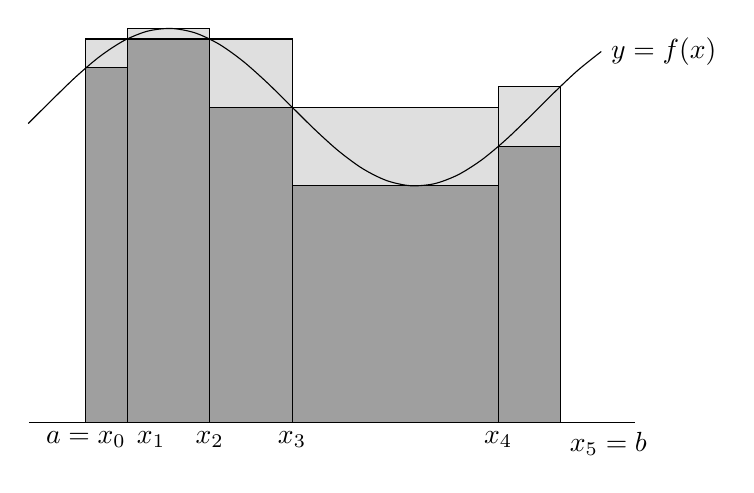
\begin{tikzpicture}
    \draw (-0.2,0)--(7.5,0);
    \filldraw[fill=lightgray!50,draw=black](pi/6,{sin(pi/6 r)+4}) rectangle (pi/3,{sin(pi/3 r)+4});
    \filldraw[fill=darkgray!50,draw=black](pi/6,0) rectangle (pi/3,{sin(pi/6 r)+4});
    \filldraw[fill=lightgray!50,draw=black](pi/3,{sin(pi/3 r)+4}) rectangle ({2*pi/3},5);
    \filldraw[fill=darkgray!50,draw=black](pi/3,0) rectangle ({2*pi/3},{sin(pi/3 r)+4});
    \filldraw[fill=lightgray!50,draw=black]({2*pi/3},{sin(pi r)+4}) rectangle (pi,{sin(2*pi/3 r)+4});
    \filldraw[fill=darkgray!50,draw=black]({2*pi/3},0) rectangle ({pi},{sin(pi r)+4});
    \filldraw[fill=lightgray!50,draw=black]({pi},3) rectangle ({11*pi/6},{sin(pi r)+4});
    \filldraw[fill=darkgray!50,draw=black]({pi},0) rectangle ({11*pi/6},3);
    \filldraw[fill=lightgray!50,draw=black]({11*pi/6},{sin(11*pi/6 r)+4}) rectangle ({25*pi/12},{sin(25*pi/12 r)+4});
    \filldraw[fill=darkgray!50,draw=black]({11*pi/6},0) rectangle ({25*pi/12},{sin(11*pi/6 r)+4});
    \draw (pi/6,0) node [below] {$a=x_0$};
    \draw (pi/3,0) node [below right] {$x_1$};
    \draw (2*pi/3,0) node [below] {$x_2$};
    \draw (pi,0) node [below] {$x_3$};
    \draw (11*pi/6,0) node [below] {$x_4$};
    \draw (25*pi/12,0) node [below right] {$x_5=b$};
    \draw [domain={-pi/15}:{27*pi/12},smooth] plot(\x, {sin(\x r) +4}) node [right]{$y=f(x)$};
  \end{tikzpicture} 
  \caption{上方和と下方和}
  \end{figure}

\deref{上方和・下方和}において，$f$は$[a,b]$で有界だから，任意の$x \in [a,b]$に対して
\[
    m \leqq f(x) \leqq M
\]
となるような$m ,M \in \mathbb{R}$が存在する．

これより，
\[
    m(b-a) \leqq L(f,P) \leqq U(f,P) \leqq M(b-a)
\]
を得て，$L(f,P)$，$U(f,P)$はともに有界であることがわかった．

\begin{definition}{細分}{細分}
	 区間$[a,b]$の分割$P^{\ast}$で，$P$の全ての分割が$P^{\ast}$の分割でもあるとき，$P^{\ast}$を$P$の細分という．
\end{definition}

\begin{prop}{細分と上方和・下方和}{細分と上方和・下方和}
	$P^{\ast}$を$P$の細分とするとき，
	\begin{align*}
		&U(f,P^{\ast})\leqq U(f,P),\\
		&L(f,P) \leqq L(f,P^{\ast})
	\end{align*}
	である．
\end{prop}

\begin{tleftbar}
	\begin{proof} 
		上方和について証明する．

		分割$P$に，$x_{i-1} \leqq x^{\ast} \leqq x_i$をみたす点$x^{\ast}$を付け加えた細分を$P^{\ast}$とする．

		このとき，$U(f,P)$と$U(f,P^{\ast})$は，前者の$M_i (x_i-x_{i-1})$の項が後者だと
		\[
			M_i ' (x^{\ast}-x_{i-1}) +M_i '' (x_i-x^{\ast})
		\]
		に変わる点のみが異なる．ただしここで$M_i ' \coloneqq \sup_{x_{i-1} \leqq x \leqq x^{\ast}} f(x)$，
		$M_i '' \coloneqq \sup_{x^\ast \leqq x \leqq  x_i} f(x)$とした．

		$M_i$，$M_i ' $，$M_i ''$の定義から
		\[
			M_i ' \leqq M_i , \quad M_i '' \leqq M_i
		\]
		なので，
		\begin{align*}
			M_i ' (x^{\ast}-x_{i-1}) +M_i '' (x_i-x^{\ast}) &\leqq M_i (x^{\ast}-x_{i-1}) + M_i(x_i -x^{\ast}) \\
			& = M_i (x_i - x_{i-1})
		\end{align*}
		となる．これよりただちに
		\[
			U(f,P^\ast) \leqq U(f,P)
		\]
		が従う．下方和についても同様である．
	\end{proof}
\end{tleftbar}
	
\begin{prop}{}{}
	有界閉区間上の連続関数は積分可能である．
\end{prop}

\begin{tleftbar}
	\begin{proof}
		$f$を$[a,b]$上で連続な関数とする．このとき，任意の$\varepsilon >0$に対して，ある$\delta >0$が存在して，任意の$x,y \in [a,b]$に対して，
		$\abs{x-y}<\delta$のとき$\abs{f(x)-f(y)}<\varepsilon$となる．

		ここで，幅が$\delta$以下の分割$P=(a_i)_{i \in \{0,1,2,\ldots,n \}}$を考える．このとき，$[a_{i-1},a_i]$の点で
		\[
			f(x_i)=m_i (f,P),\quad f(y_i)=M_i (f,P)
		\]
		なるものが存在する．

		$\abs{x_i-y_i}\leqq \delta$であるから，$f(y_i)-f(x_i)<\varepsilon$となる．よって
		\[
			U(f,P)-L(f,P) = \sum_{i=1}^{n} ( f(y_i)-f(x_i) ) (a_i-a_{i-1}) <(b-a)\varepsilon 
		\]
		となる．

		ここで，$L(f,P) \leqq L(f) \leqq U(f) \leqq U(f,P)$なので，$L(f)=U(f)$となり，$f$は積分可能である．
	\end{proof}
\end{tleftbar}
\phantomsection
\section{定積分の性質}

\begin{prop}{}{}
	$f$が連続であるならば，
	\[
		\int_{a}^{b} f(x)\, dx = \int_{a}^{c} f(x)\, dx + \int_{c}^{b} f(x)\, dx
	\]
	が成立する．
\end{prop}

証明略．

\begin{prop}{線型性}{線型性}
	連続関数$f$，$g$に対して，
	\[
		\int_{a}^{b} (kf(x)+lg(x))\, dx = k\int_{a}^{b} f(x)\, dx + l\int_{a}^{b} g(x)\, dx
	\]
	が成立する．
\end{prop}

証明略．


\begin{definition}{リーマン和}{リーマン和}
	有界閉区間$[a,b]$上の有界関数$f$に対して，$P=(x_i)_{i \in \{0,1,2,\ldots,n\}}$を分割とする．

	さらには，$\xi_i \in [x_{i-1},x_i]$を適当に選ぶ．
	
	このとき，
	\[
		\sum_{i=1}^{n} f(\xi_i)(x_i - x_{i-1})
	\]
	を分割$P$と代表点$(\xi_i)_{i \in \{1,2,\ldots,n\} }$による$f$のリーマン和といい，
	\[
		R(f,P,\xi)
	\]
	と表す．
\end{definition}


\part*{\texorpdfstring{積分($n$次元)}{積分(n次元)}}

\begin{definition}{}{}
	$n$次元の有界閉区間
	\begin{align*}
	I&=[a_1,b_1] \times [a_2,b_2] \times \cdots \times [a_n,b_n] \\
	& = \{ (x_1,x_2,\ldots,x_n) \mid a_i \leqq x_i \leqq b_i , i \in \{1,2,\dots,n \} \}
	\end{align*} 
	の$n$次元体積を，
	\[
		v(I) = \prod_{i=1}^{n} (b_i-a_i)
	\]
	と定義する．
\end{definition}

\begin{definition}{}{}
	区間$I$に対して，集合 $D(I)$を
	\[
		D(I) = \{ (x_i)_{i \in \{0,1,\ldots,n \}} \mid a=x_0 < x_1<\dots < x_n =b , n \in \mathbb{N} \}
	\]
	とする．
\end{definition}

\begin{prop}{}{}
	$D(I)$は $(a,b)$の有限部分集合全体の集合$P((a,b))$と一対一に対応する．ただし，$a=b$のときは$a$を分点とする分割を考える．
\end{prop}

\begin{tleftbar}
	\begin{proof}
		写像$f$を
		\[
			f \colon D(I) \ni (x_i)_{i \in \{0,1,\ldots,n \}} \mapsto (x_i)_{i \in \{1,\ldots,n-1 \}} \in P((a,b))
		\]
		とする．このとき，$f$が全単射であることを示す．
		\begin{description}
			\item[単射であること] まず，$(x_i)_{i \in \{0,1,\ldots,n \}} \neq (y_i)_{i \in \{0,1,\ldots,n\}}$とする． 
			このとき，ある$j \in \{0,1,\ldots,n \}$に対して，$ x_j \ne y_j $である．特に$ j \ne 0$かつ$j \ne n$のとき，
			\begin{align*} 
				& (x_i)_{i \in \{1,2,\ldots,n-1 \}} \neq (y_i)_{i \in \{1,2,\ldots,n-1\}}, \\
				& \therefore ~ f((x_i)_{i \in \{0,1,\ldots,n \}}) \neq f((y_i)_{i \in \{0,1,\ldots,n\}})
			\end{align*} 
			となるため，$f$は単射である．
			\item[全射であること] 任意の$(x_i)_{i \in \{1,\ldots,n-1 \}} \in P((a,b))$に対して，$a$および$b$を初項と末項に設定し，
			有限点列として
			\[
			(a,x_1,x_2,\ldots,x_{n-1},b)
			\]
			を考えると，これは$(x_0,x_1,\ldots,x_{n-1},x_n)$に等しい．ゆえにこのとき
			\[
			f((x_i)_{i \in \{0,1,\ldots,n\}})=(x_i)_{i \in \{1,\ldots,n-1 \}}
			\]
			となる$(x_i)_{i \in \{1,\ldots,n-1 \}} \in D(I)$が存在し，$f$は全射である．
		\end{description}
		以上の考察により，$f$は単射かつ全射，すなわち全単射である．
	\end{proof}
\end{tleftbar}
